%%%%%%%%%%%%%%%%%%%%%%%%%%%%%%%%%%%%%%%%%%%%%%%%
%% Intro to LaTeX and Template for Homework Assignments
%% Quantitative Methods in Political Science
%% University of Mannheim
%% Fall 2019
%%%%%%%%%%%%%%%%%%%%%%%%%%%%%%%%%%%%%%%%%%%%%%%%

% created by Marcel Neunhoeffer & Sebastian Sternberg


% This template and tutorial will help you to write up your homework. It will also help you to use Latex for other assignments than this course's homework.

%%%%%%%%%%%%%%%%%%%%%%%%%%%%%%%%%%%%%%%%%%%%%%%%
% Before we get started
%%%%%%%%%%%%%%%%%%%%%%%%%%%%%%%%%%%%%%%%%%%%%%%%

% Make an account on overleaf.com and get started. No need to install anything.

%%%%%%%%%%%%%%%%%%%%%%%%%%%%%%%%%%%%%%%%%%%%%%%%
% Or if you want it the nerdy way...
% INSTALL LATEX: Before we can get started you need to install LaTeX on your computer.
				% Windows: http://miktex.org/download
				% Mac:         http://www.tug.org/mactex/mactex-download.html	
				% There a many more different LaTeX editors out there for both operating systems. I use TeXworks because it looks the same on Windows and Mac.
				

% SAVE THE FILE: The first thing you need to do is to save your LaTeX file in a directory as a .tex file. You will not be able to do anything else unless your file is saved. I suggest to save the .tex file in the same folder with your .R script and where you will save your plots from R to. Let's call this file template_homework1.tex and save it in your Week 1 folder.


% COMPILE THE FILE: After setting up your file, using your LaTeX editor (texmaker, texshop), you can compile your document using PDFLaTeX.
	% Compiling your file tells LaTeX to take the code you have written and create a pdf file
	% After compiling your file, in your directory will appear four new files, including a .pdf file. This is your output document.
	% It is good to compile your file regularly so that you can see how your code is translating into your document.
	
	
% ERRORS: If you get an error message, something is wrong in your code. Fix errors before they pile up!
	% As with error messages in R, google the exact error message if you have a question!
%%%%%%%%%%%%%%%%%%%%%%%%%%%%%%%%%%%%%%%%%%%%%%%%


% Now again for everyone...

% COMMANDS: 
	% To do anything in LaTeX, you must use commands
	% Commands tell LaTeX when to start your document, how you want your document to look, and how to format your document
	% Commands ALWAYS begin with a backslash \

% Everything following the % sign is a comment and will not be used by Latex to compile your document.
% This is very similar to # comments in R.

% Every .tex file usually consists of four parts.
% 1. Document Class
% 2. Packages
% 3. Header
% 4. Your Document

%%%%%%%%%%%%%%%%%%%%%%%%%%%%%%%%%%%%%%%%%%%%%%%%
% 1. Document Class
%%%%%%%%%%%%%%%%%%%%%%%%%%%%%%%%%%%%%%%%%%%%%%%%
 
 % The first command you will always have will declare your document class. This tells LaTeX what type of document you are creating (article, presentation, poster, etc). 
% \documentclass is the command
% in {} you specify the type of document
% in [] you define additional parameters
 
\documentclass[a4paper,12pt]{article} % This defines the style of your paper

% We usually use the article type. The additional parameters are the format of the paper you want to print it on and the standard font size. For us this is a4paper and 12pt.

%%%%%%%%%%%%%%%%%%%%%%%%%%%%%%%%%%%%%%%%%%%%%%%%
% 2. Packages
%%%%%%%%%%%%%%%%%%%%%%%%%%%%%%%%%%%%%%%%%%%%%%%%

% Packages are libraries of commands that LaTeX can call when compiling the document. With the specialized commands you can customize the formatting of your document.
% If the packages we call are not installed yet, TeXworks will ask you to install the necessary packages while compiling.

% First, we usually want to set the margins of our document. For this we use the package geometry. We call the package with the \usepackage command. The package goes in the {}, the parameters again go into the [].
\usepackage[top = 2.5cm, bottom = 2.5cm, left = 2.5cm, right = 2.5cm]{geometry} 

% Unfortunately, LaTeX has a hard time interpreting German Umlaute. The following two lines and packages should help. If it doesn't work for you please let me know.
\usepackage[T1]{fontenc}
\usepackage[utf8]{inputenc}

% The following two packages - multirow and booktabs - are needed to create nice looking tables.
\usepackage{multirow} % Multirow is for tables with multiple rows within one cell.
\usepackage{booktabs} % For even nicer tables.

% As we usually want to include some plots (.pdf files) we need a package for that.
\usepackage{graphicx} 

% The default setting of LaTeX is to indent new paragraphs. This is useful for articles. But not really nice for homework problem sets. The following command sets the indent to 0.
\usepackage{setspace}
\setlength{\parindent}{0in}

% Package to place figures where you want them.
\usepackage{float}

% The fancyhdr package let's us create nice headers.
\usepackage{fancyhdr}


%%%%%%%%%%%%%%%%%%%%%%%%%%%%%%%%%%%%%%%%%%%%%%%%
% 3. Header (and Footer)
%%%%%%%%%%%%%%%%%%%%%%%%%%%%%%%%%%%%%%%%%%%%%%%%

% To make our document nice we want a header and number the pages in the footer.

\pagestyle{fancy} % With this command we can customize the header style.

\fancyhf{} % This makes sure we do not have other information in our header or footer.

\lhead{\footnotesize TRABALHO PRÁTICO N.01}% \lhead puts text in the top left corner. \footnotesize sets our font to a smaller size.

%\rhead works just like \lhead (you can also use \chead)
\rhead{\footnotesize Gabrich Navarro , Murta Lopes} %<---- Fill in your lastnames.

% Similar commands work for the footer (\lfoot, \cfoot and \rfoot).
% We want to put our page number in the center.
\cfoot{\footnotesize \thepage} 


%%%%%%%%%%%%%%%%%%%%%%%%%%%%%%%%%%%%%%%%%%%%%%%%
% 4. Your document
%%%%%%%%%%%%%%%%%%%%%%%%%%%%%%%%%%%%%%%%%%%%%%%%

% Now, you need to tell LaTeX where your document starts. We do this with the \begin{document} command.
% Like brackets every \begin{} command needs a corresponding \end{} command. We come back to this later.

\begin{document}


%%%%%%%%%%%%%%%%%%%%%%%%%%%%%%%%%%%%%%%%%%%%%%%%
%%%%%%%%%%%%%%%%%%%%%%%%%%%%%%%%%%%%%%%%%%%%%%%%

%%%%%%%%%%%%%%%%%%%%%%%%%%%%%%%%%%%%%%%%%%%%%%%%
% Title section of the document
%%%%%%%%%%%%%%%%%%%%%%%%%%%%%%%%%%%%%%%%%%%%%%%%

% For the title section we want to reproduce the title section of the Problem Set and add your names.

\thispagestyle{empty} % This command disables the header on the first page. 

\begin{tabular}{p{15.5cm}} % This is a simple tabular environment to align your text nicely 
{\large \bf TRABALHO PRÁTICO N.01} \\
Pontifícia Universidade Católica de Minas Gerais \\ 11/2023 \\
\hline % \hline produces horizontal lines.
\\
\end{tabular} % Our tabular environment ends here.

\vspace*{0.3cm} % Now we want to add some vertical space in between the line and our title.

\begin{center} % Everything within the center environment is centered.
	{\Large \bf Fundamentos Teóricos da Computação} % <---- Don't forget to put in the right number
	\vspace{2mm}
	
        % YOUR NAMES GO HERE
	{\bf Marcus Navarro Gabrich / Matrícula: 700185  \\ Rafael Murta Lopes / Matrícula: 690213} % <---- Fill in your names here!

\end{center}  

\vspace{0.4cm}

%%%%%%%%%%%%%%%%%%%%%%%%%%%%%%%%%%%%%%%%%%%%%%%%
%%%%%%%%%%%%%%%%%%%%%%%%%%%%%%%%%%%%%%%%%%%%%%%%

% Up until this point you only have to make minor changes for every week (Number of the homework). Your write up essentially starts here.

\section{Introdução}

Este trabalho centra-se na importância das transformações de gramáticas e na implementação de algoritmos para converter gramáticas em Forma Normal de Chomsky (FNC) e Segunda Forma Normal (2NF). As transformações gramaticais são fundamentais no contexto de linguagens formais e gramáticas, desempenhando um papel crucial na análise e manipulação de estruturas gramaticais. A capacidade de representar as regras de uma gramática em formas normais específicas simplifica significativamente o processo de compreensão e processamento, proporcionando vantagens na resolução de diversos problemas associados às linguagens formais.
\\
A Forma Normal de Chomsky é uma representação especial de uma gramática livre de contexto em que todas as produções têm um formato específico, facilitando a aplicação de algoritmos de análise sintática e simplificando a interpretação da linguagem definida pela gramática. A Segunda Forma Normal, por sua vez, é uma adaptação para gramáticas em que as produções são limitadas a ter no máximo dois não-terminais do lado direito, contribuindo para uma estrutura mais organizada e eficiente em determinadas aplicações.
\\
Ao abordar a implementação de algoritmos específicos para realizar essas transformações, este trabalho busca fornecer uma contribuição prática para a compreensão e aplicação dessas técnicas. Os algoritmos CYK (Cocke-Younger-Kasami) e uma versão modificada denominada \texttt{ModifiedCyk} são apresentados para verificar se uma gramática gera uma determinada entrada, sendo essenciais na validação e análise de expressões em linguagens formais. As classes \texttt{ChomskyNormalForm} e \texttt{SecondNormalForm} detalham os processos de conversão de gramáticas para FNC e 2NF, respectivamente, destacando a importância dessas formas normais na simplificação e otimização de estruturas gramaticais.

Assim, ao compreender a relevância das transformações de gramáticas e explorar a implementação de algoritmos específicos, este trabalho visa contribuir para a compreensão prática e teórica das linguagens formais, oferecendo uma base sólida para a aplicação dessas técnicas em diversas áreas, como compiladores, processamento de linguagem natural e análise sintática.



\section{Implementações de Código}

Descrevemos abaixo as implementações de código desenvolvidas para realizar transformações em gramáticas.

\subsection{Leitura de Regras Gramaticais}

A leitura das regras gramaticais é a primeira etapa do processo a ser feito após criar uma gramática. Em nossa implementação os terminais, variáveis e regras de produção são definidos pela função \texttt{readGramatica} presente na classe \texttt{Gramatica}.

\subsubsection{Função \texttt{loadModel}}

Essa é a única função chamada pela \texttt{readGramatica} recebendo o caminho para o arquivo de texto contendo os terminais, estados e regras de produção da gramática de uma forma amigável ao usuário e retorna os terminais, variáveis e regras de produção já tratados de forma a facilitar o seu uso no programa. Para isso o arquivo de texto é aberto e é realizado uma pré limpeza da entrada, com uma variável K contendo os terminais, uma variável V contendo as variáveis e uma variável P contendo as regras de produção. A função \texttt{cleanAlphabet} é chamada para as variáveis K e V e \texttt{cleanProductions} chamada para a variável P.

\subsubsection{Função \texttt{cleanProductions}}
Essa função recebe uma string contendo as regras de produção e retorna uma lista de tuplas representando as produções.

\subsubsection{Função \texttt{cleanAlphabet}}
Essa função recebe uma string contendo a uma sequência de terminais ou estados e retorna uma lista de símbolos.

\subsubsection{Funcionalidade e Importância}

A funcionalidade das funções de leitura de regras gramaticais é fundamental para o fluxo de trabalho subsequente. Ela simplifica e automatiza a leitura de regras gramaticais a partir de um arquivo externo, garantindo que essas regras estejam prontas para serem processadas pelos algoritmos de transformação gramatical. A correta execução desta etapa inicial é crucial para assegurar a qualidade e consistência das análises e transformações gramaticais realizadas ao longo do projeto.

\subsection{Implementação de Formas Normais de Chomsky e Segunda Forma Normal}

Essas formas normais são essenciais para simplificar e otimizar as regras gramaticais, facilitando análises sintáticas e processamentos subsequentes. Nesta seção, examinaremos detalhadamente a implementação dessa funcionalidade crucial.

\subsubsection{\texttt{ChomskyNormalForm}}

A função \texttt{cfgToCnf} é responsável pela conversão de gramáticas para a Forma Normal de Chomsky. Ela funciona do seguinte modo:
Recebe uma gramática, logo em seguida chama a função \texttt{methods.defineVariables} que organiza as variáveis ainda não utilizadas para facilitar o uso. Depois chama as funções de conversão \texttt{methods.START}, \texttt{methods.TERM} \texttt{methods.BIN}, \texttt{methods.DEL} e \texttt{methods.UNIT}. Por fim chama a função \texttt{methods.startingRuleFirst} que move a regra inicial para o início da lista de regras.

\subsubsection{\texttt{SecondNormalForm}}

A função \texttt{cfgTo2nf} é responsável pela conversão de gramáticas para a Segunda Forma Normal. Ela funciona de modo semelhante ao da função \texttt{cfgToCnf}, mas como diferença ao invés de utilizar as 5 funções de conversão, utiliza apenas a \texttt{methods.BIN} e não tem a necessidade de chamar a \texttt{methods.startingRuleFirst}.

\subsubsection{Funcionalidade e Importância}

A implementação dessas funções é crucial para o processo de normalização de gramáticas, proporcionando uma estrutura que simplifica e otimiza as regras, preparando-as para análises sintáticas e processamentos subsequentes. A Forma Normal de Chomsky e a Segunda Forma Normal são padrões fundamentais em linguagens formais, e a correta execução desses algoritmos é essencial para garantir a consistência e a eficácia das transformações realizadas nas gramáticas.


\subsection{Algoritmos para Verificação de Gramáticas}

O arquivo \texttt{algorithms.py} contém implementações dos algoritmos fundamentais para a verificação de gramáticas. Estes algoritmos desempenham um papel crucial no contexto de linguagens formais e gramáticas, oferecendo meios eficazes para determinar se uma dada gramática pode gerar uma determinada sequência de símbolos. Nesta seção, abordaremos detalhadamente as duas principais classes contidas neste arquivo: \texttt{Cyk} e \texttt{ModifiedCyk}.

\subsubsection{\texttt{Cyk}}

A classe \texttt{Cyk} implementa o algoritmo Cocke-Younger-Kasami (CYK), utilizado para verificar se uma gramática gera uma determinada sequência de símbolos. O método principal é o \texttt{run}.

O método utiliza uma tabela dinâmica para verificar se a gramática definida pelas regras de entrada pode gerar a sequência de símbolos fornecida. O algoritmo é eficiente e amplamente utilizado em análise sintática.

\subsubsection{\texttt{ModifiedCyk}}

A classe \texttt{ModifiedCyk} implementa uma versão modificada do algoritmo CYK. Seu método principal também é o \texttt{run}, mas antes de ser chamado é necessário chamar o \texttt{methods.anulavel} que retorna as variáveis anuláveis.

Esta versão modificada se baseia na versão original, mas utiliza de três funções extras, a \texttt{inverseUnitGraph} que recebe a gramática e as variáveis anuláveis e retorna o grafo de unidade inverso, a \texttt{discoverReach} que recebe o grafo e a lista de palavras e retorna a lista de símbolos alcançáveis e a \texttt{dfs} que recebe um grafo e o nó inicial e retorna a lista de nós alcançáveis.

\subsubsection{Funcionalidade e Importância}

Os algoritmos implementados em \texttt{algorithms.py} são essenciais para a verificação prática de gramáticas. Eles oferecem meios para determinar se uma gramática pode gerar uma determinada sequência de símbolos, sendo fundamentais em processos de análise sintática e transformações gramaticais. O algoritmo CYK, em particular, é amplamente utilizado e reconhecido na área de linguagens formais.

\section{Experimentos e Resultados}

Realizamos experimentos utilizando diversas gramáticas de tamanhos variados como entrada para avaliar a eficácia das transformações implementadas. Os resultados como se pode ver na Figura 1 demonstram o ganho de performance do cyk modificado frente o original, que gasta apenas 70\% do tempo originalmente gasto.

\begin{figure}[!h]
\centering
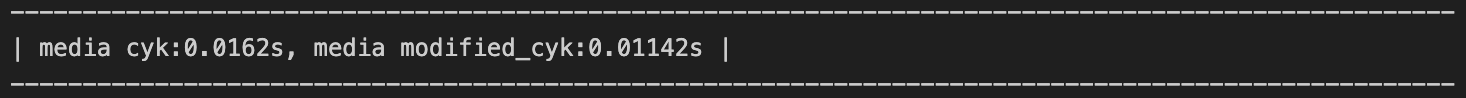
\includegraphics[width=16cm]{media_tempo.png}
\caption{Média dos tempos dos algoritmos.}
\label{fig:Media_img}
\end{figure}

Os testes foram realizados para as seguintes gramaticas:

\section*{Gramática 1}
\textbf{Variáveis:}
\[
['S', 'A', 'B', 'C', 'D', 'E', 'F', 'G', 'H', 'I', 'J']
\]

\textbf{Terminais:}
\[
['a', 'b']
\]

\textbf{Regras:}
\begin{align*}
S &\to A \mid B \\
A &\to a E \mid \varepsilon \\
B &\to a F \mid b I \\
C &\to \varepsilon \\
D &\to b J \\
E &\to a E E \mid a F G \mid b C \\
F &\to a E F \mid a F H \mid b D \\
G &\to b \\
H &\to b D \\
I &\to a E F G \mid b \\
J &\to a F H \mid b D \\
\end{align*}

\textbf{Resultados:}
\begin{itemize}
    \item Utilizando CYK: "aaabbb" pertence à gramática \\
    Utilizando CYK Modificado: "aaabbb" pertence à gramática \\
    Tempo de execução CYK: 0.00028 \\
    Tempo de execução CYK Modificado: 0.0003 \\
    
    \item Utilizando CYK: "aaaaaaaaaaaaaaabbbbbbbbbbbbbbbb" não pertence à gramática \\
    Utilizando CYK Modificado: "aaaaaaaaaaaaaaabbbbbbbbbbbbbbbb" não pertence à gramática \\
    Tempo de execução CYK: 0.01309 \\
    Tempo de execução CYK Modificado: 0.01151 \\
    
    \item Utilizando CYK: "ab" pertence à gramática \\
    Utilizando CYK Modificado: "ab" pertence à gramática \\
    Tempo de execução CYK: 0.00016 \\
    Tempo de execução CYK Modificado: 0.00011 \\
\end{itemize}

\section*{Gramática 2}
\textbf{Variáveis:}
\[
['E']
\]

\textbf{Terminais:}
\[
['t', '+', '*', '(', ')']
\]

\textbf{Regras:}
\[
E \to E + E \mid E \mid E * E \mid E \mid ( E ) \mid t
\]

\textbf{Resultados:}
\begin{itemize}
    \item Utilizando CYK: "t+t+t+t+t+t+(t)" pertence à gramática \\
    Utilizando CYK Modificado: "t+t+t+t+t+t+(t)" pertence à gramática \\
    Tempo de execução CYK: 0.00168 \\
    Tempo de execução CYK Modificado: 0.00126 \\
    
    \item Utilizando CYK: "()" não pertence à gramática \\
    Utilizando CYK Modificado: "()" não pertence à gramática \\
    Tempo de execução CYK: 0.00029 \\
    Tempo de execução CYK Modificado: 4e-05 \\
    
    \item Utilizando CYK: "(t)+t" pertence à gramática \\
    Utilizando CYK Modificado: "(t)+t" pertence à gramática \\
    Tempo de execução CYK: 0.00087 \\
    Tempo de execução CYK Modificado: 0.00012 \\
\end{itemize}

\section*{Gramática 3}
\textbf{Variáveis:}
\[
['P', 'Z']
\]

\textbf{Terminais:}
\[
['0', '1']
\]

\textbf{Regras:}
\begin{align*}
P &\to 0 P 0 \mid 1 P 1 \mid 0 \mid 1 \mid Z \\
Z &\to \varepsilon
\end{align*}

\textbf{Resultados:}
\begin{itemize}
    \item Utilizando CYK: "0000001111111" pertence à gramática \\
    Utilizando CYK Modificado: "0000001111111" não pertence à gramática \\
    Tempo de execução CYK: 0.00044 \\
    Tempo de execução CYK Modificado: 0.00042 \\
    
    \item Utilizando CYK: "1" pertence à gramática \\
    Utilizando CYK Modificado: "1" pertence à gramática \\
    Tempo de execução CYK: 5e-05 \\
    Tempo de execução CYK Modificado: 3e-05 \\
\end{itemize}

\section*{Gramática 4}
\textbf{Variáveis:}
\[
['E', 'T', 'F']
\]

\textbf{Terminais:}
\[
['t', '+', '*', '(', ')']
\]

\textbf{Regras:}
\begin{align*}
E &\to E + T \mid T \\
T &\to T * F \mid F \\
F &\to ( E ) \mid t
\end{align*}

\textbf{Resultados:}
\begin{itemize}
    \item Utilizando CYK: "t+t+t+t+t+t+(t)" pertence à gramática \\
    Utilizando CYK Modificado: "t+t+t+t+t+t+(t)" pertence à gramática \\
    Tempo de execução CYK: 0.0007 \\
    Tempo de execução CYK Modificado: 0.00061 \\
    
    \item Utilizando CYK: "()" não pertence à gramática \\
    Utilizando CYK Modificado: "()" não pertence à gramática \\
    Tempo de execução CYK: 9e-05 \\
    Tempo de execução CYK Modificado: 3e-05 \\
\end{itemize}

\textbf{Resultados finais:}
\begin{itemize}
    \item Media de tempo de execução CYK: 0.01798
    \item Media de tempo de execução CYK Modificado 0.01207
\end{itemize}

\section{Conclusão}

Este trabalho apresentou implementações dos algoritmos CYK e CYK Modificado. Os experimentos realizados demonstram o ganho de performance proposto pelo CYK Modificado. No entanto, vale ressaltar que existem limitações e possíveis melhorias que podem ser investigadas em trabalhos futuros.


\end{document}
